% !TeX spellcheck = ru_RU
% !TEX root = vkr.tex

\section{Особенности реализации}

\subsection{Используемый стек технологий}

\textbf{Язык программирования и среда выполнения.} В качестве основного языка реализации выбран \texttt{Python} \cite{Python} версии 3.12 и выше. Выбор обусловлен следующими факторами:
\begin{itemize}
    \item Использование языка разработчиками алгоритмов;
    \item Наличие мощных библиотек для научных вычислений (\texttt{NumPy} \cite{NumPy}) и визуализации (\texttt{Matplotlib} \cite{Matplotlib});
    \item Развитая экосистема веб-фреймворков, в частности \texttt{Django} \cite{Django}, используемого для реализации веб-интерфейса;
    \item Возможность динамической загрузки пользовательских модулей, что критически важно для поддержки расширяемости системы пользовательскими алгоритмами.
\end{itemize}

\textbf{Веб-фреймворк и бэкенд.} Для реализации серверной части и веб-интерфейса используется \texttt{Django 5.2.7}. Фреймворк обеспечивает:
\begin{itemize}
    \item ORM для работы с базой данных и моделями пользователей;
    \item Встроенную систему аутентификации и авторизации;
    \item Маршрутизацию URL и систему шаблонов;
    \item Административную панель для управления пользователями и алгоритмами.
\end{itemize}

В качестве СУБД в проекте используется \texttt{SQLite3} \cite{sqlite3} (на этапе разработки) с возможностью переключения на \texttt{PostgreSQL} \cite{PostgreSQL} через драйвер \texttt{psycopg2} \cite{psycopg2}.

\textbf{Библиотеки для научных вычислений и визуализации.}
Для реализации алгоритмов, симуляции и визуализации резульатов был использован ряд популярных в индустрии и науке библиотек: 
\begin{itemize}
    \item \texttt{NumPy 2.3.3} --- для работы с многомерными массивами, выполнения матричных операций и линейно-алгебраических преобразований;
    \item \texttt{Matplotlib 3.10.6} --- для построения графиков траекторий движения целей и визуализации сходимости ошибок оценок;
    \item \texttt{SciPy} \cite{SciPy} (через зависимости \texttt{NumPy}) --- для вычисления собственных чисел матриц и решения линейных систем.
\end{itemize}

\textbf{Динамическая загрузка пользовательских алгоритмов.} Ключевой особенностью системы является возможность загрузки пользовательских алгоритмов отслеживания. Для этого используется модуль \texttt{importlib.util}, который позволяет:
\begin{enumerate}
    \item Динамически компилировать загруженный Python-файл;
    \item Проверять наследование от базового класса \texttt{TrackingAlgorithm};
    \item Загружать модуль в память и вызывать его методы в процессе симуляции.
\end{enumerate}
Загруженные алгоритмы сохраняются в модели \texttt{CustomAlgorithm} и ассоциируются с конкретным пользователем.

\textbf{Фронтенд и визуализация.} Для отображения веб-интерфейса используются:
\begin{itemize}
    \item \texttt{Bootstrap 5.3.0} \cite{Bootstrap} --- для адаптивного оформления страниц;
    \item Встроенная система шаблонов \texttt{Django} с пользовательскими фильтрами;
    \item Генерация графиков в формате PNG с последующим кодированием в Base64 для встраивания в HTML-страницы без сохранения на диск.
\end{itemize}

\textbf{Тестирование.} Для обеспечения надежности системы используется фреймворк \texttt{pytest 7.4.0} \cite{pytest} с расширением \texttt{pytest-django 4.5.2} \cite{pytestdjango}. Написаны следующие категории тестов:
\begin{itemize}
    \item Модульные тесты алгоритмов;
    \item Интеграционные тесты взаимодействия симуляции и алгоритмов;
    \item Тесты с использованием мок-объектов для изоляции компонентов.
\end{itemize}

\textbf{Инструменты разработки и CI/CD.} Проект интегрирован с платформой \texttt{GitHub Actions} \cite{actions}, что обеспечивает:
\begin{itemize}
    \item Автоматическую проверку стиля кода (линтер);
    \item Запуск тестов при каждом пуше в репозиторий;
\end{itemize}


\subsection{Симуляция}
Процесс симуляции начинается с конфигурирования параметров через веб-интерфейс (рис. \ref{fig:setup}). Пользователь задаёт длительность симуляции, количество сенсоров, число линейных и случайных целей, а также количество запусков для статистической достоверности результатов. Для имитации реальных условий предусмотрена возможность добавления шума в измерения расстояний (равномерного или гауссовского) с настраиваемыми параметрами.

\begin{figure}[H]
    \centering
    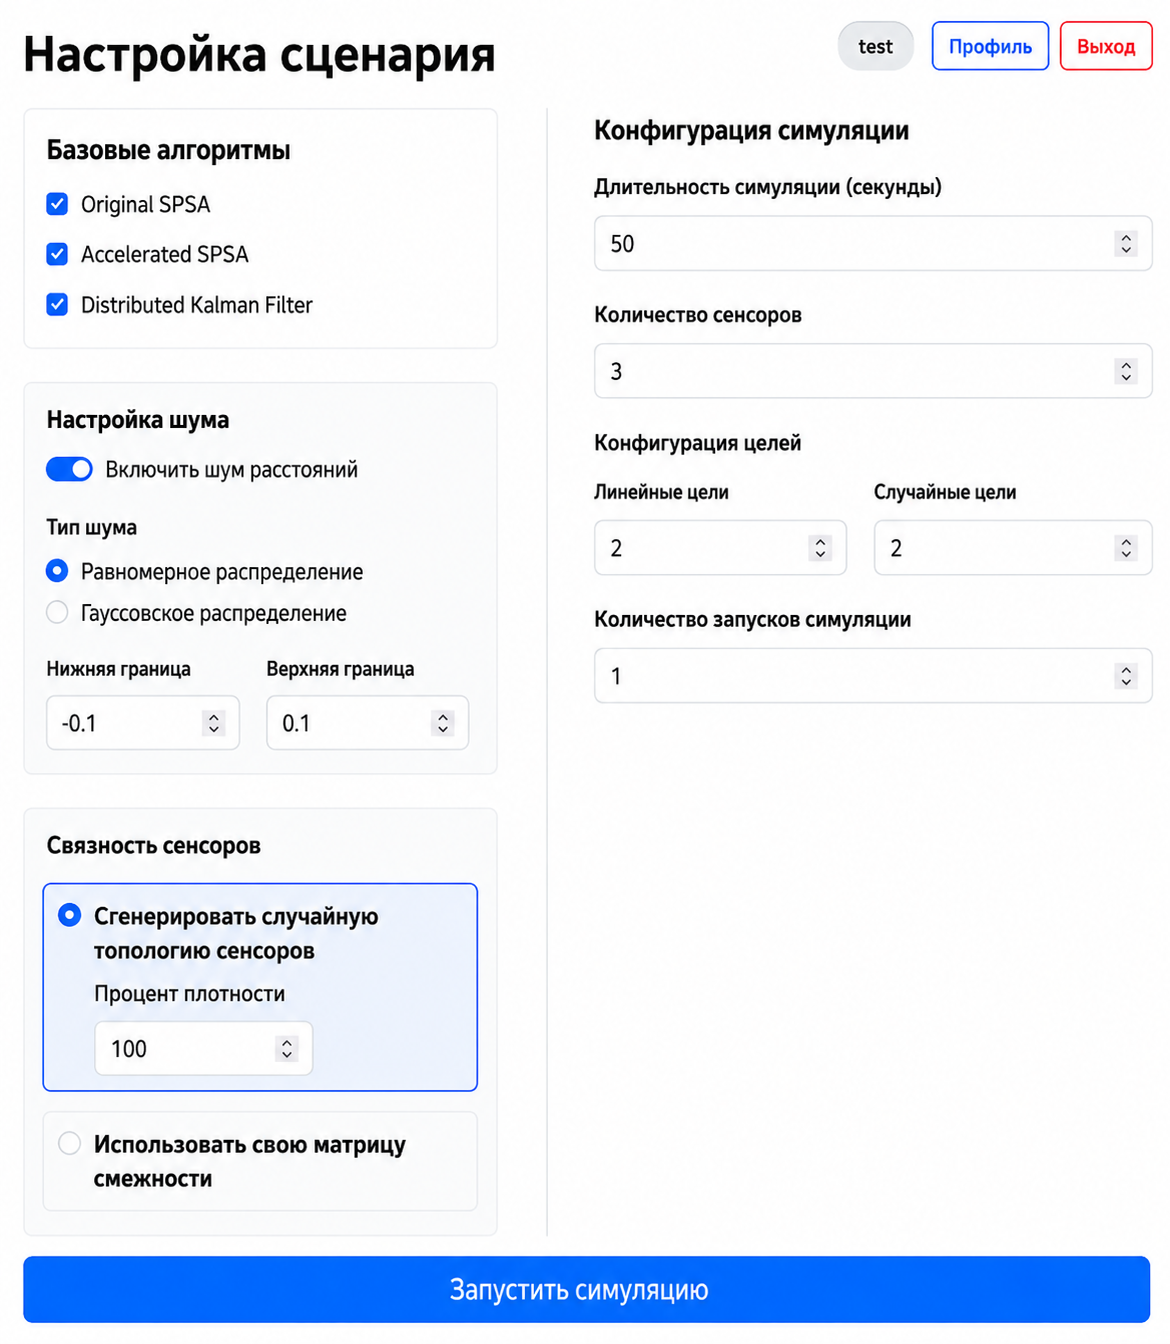
\includegraphics[width=0.8\textwidth]{setup.png}
    \caption{Интерфейс конфигурирования параметров симуляции}
    \label{fig:setup}
\end{figure}

После запуска симуляции генерируются траектории движения целей (линейные или со случайным блужданием). Для каждого момента времени вычисляются истинные расстояния от каждого сенсора до каждой цели, после чего к ним применяется выбранная модель шума. Эти данные последовательно подаются на вход каждому из выбранных алгоритмов отслеживания, которые производят оценки позиций целей. Поддерживается как однократный запуск, так и пакетное выполнение нескольких сохранённых конфигураций для сравнительного анализа.

\subsection{Пользовательские аккаунты и алгоритмы}
Система поддерживает регистрацию пользователей с возможностью сохранения персональных конфигураций симуляции и загрузки собственных алгоритмов отслеживания. Пользовательские алгоритмы должны наследоваться от базового класса \texttt{TrackingAlgorithm} и реализовывать метод \texttt{run\_n\_iterations}. При загрузке файла производится проверка корректности интерфейса.

В проекте реализованы три встроенных алгоритма, описанные далее в работе:
\begin{itemize}
    \item \textbf{Алгоритм на основе SPSA (Simultaneous Perturbation Stochastic Approximation — стохастическая аппроксимация одновременного возмущения) + консенсус \cite{Original_SPSA}};
    \item \textbf{Ускоренный алгоритм на основе SPSA + консенсус \cite{Accelerated_SPSA}};
    \item \textbf{Распределенный фильтр Калмана \cite{Distributed_Kalman}}.
\end{itemize}

Пользовательские алгоритмы загружаются через веб-форму, после чего становятся доступными для выбора в интерфейсе настройки симуляции наравне со встроенными.

\subsection{Визуализация}
Результаты симуляции представляются в виде набора графиков, генерируемых с использованием библиотеки \texttt{matplotlib}. Для каждого запуска отображаются:

\begin{itemize}
    \item Траектории истинного движения целей и оценки, полученные каждым алгоритмом (рис. \ref{fig:mutual}).
    \item Графики сходимости ошибки, усреднённой по всем сенсорам для каждой цели.
\end{itemize}

\begin{figure}[H]
    \centering
    \makebox[\textwidth][c]{%
        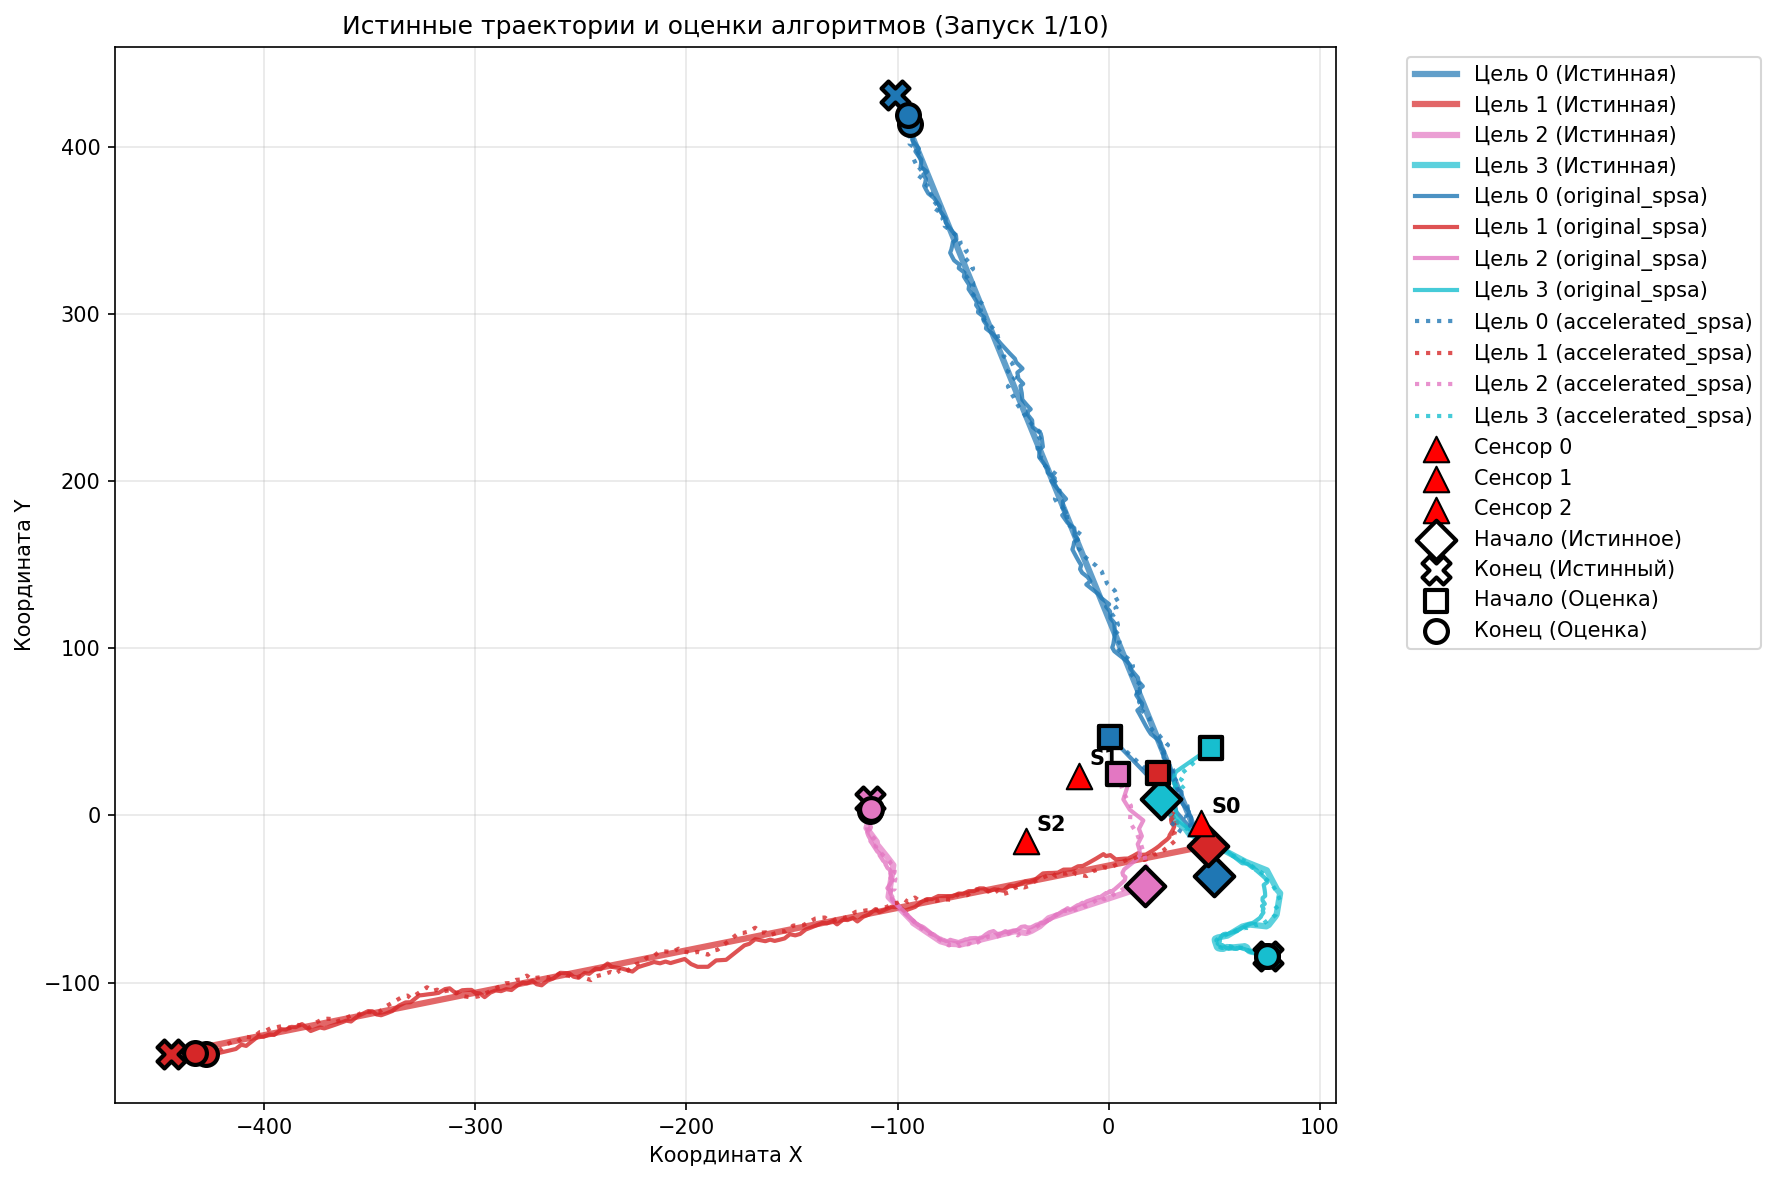
\includegraphics[width=0.58\textwidth]{mut_left_part.png}%
        \hfill
        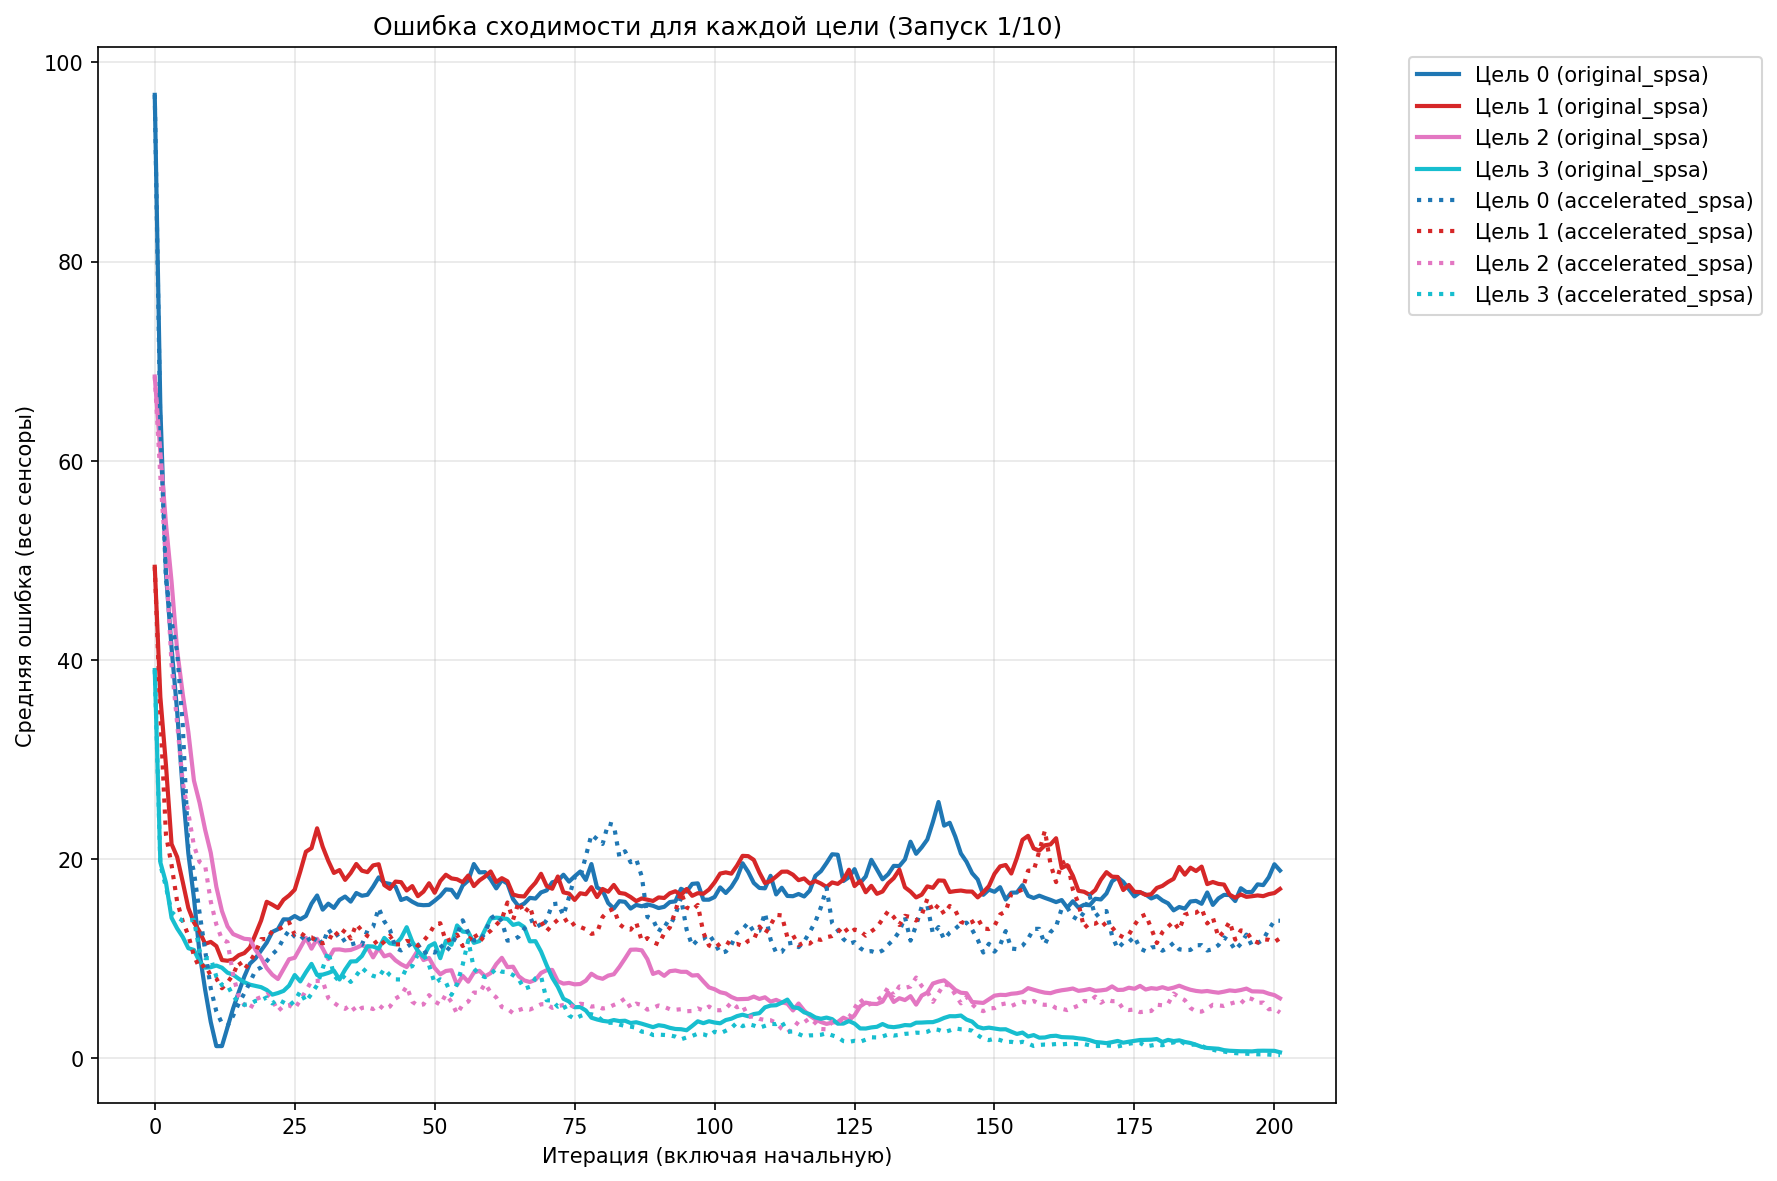
\includegraphics[width=0.58\textwidth]{mut_right_part.png}%
    }
    \caption{Совмещённые траектории и ошибки для всех алгоритмов}
    \label{fig:mutual}
\end{figure}

Для детального анализа предусмотрен режим просмотра отдельных комбинаций сенсора и цели, где показывается траектория оценки конкретного сенсора за выбранной целью и соответствующая динамика ошибки (рис. \ref{fig:specific}).

\begin{figure}[H]
    \centering
    \makebox[\textwidth][c]{%
        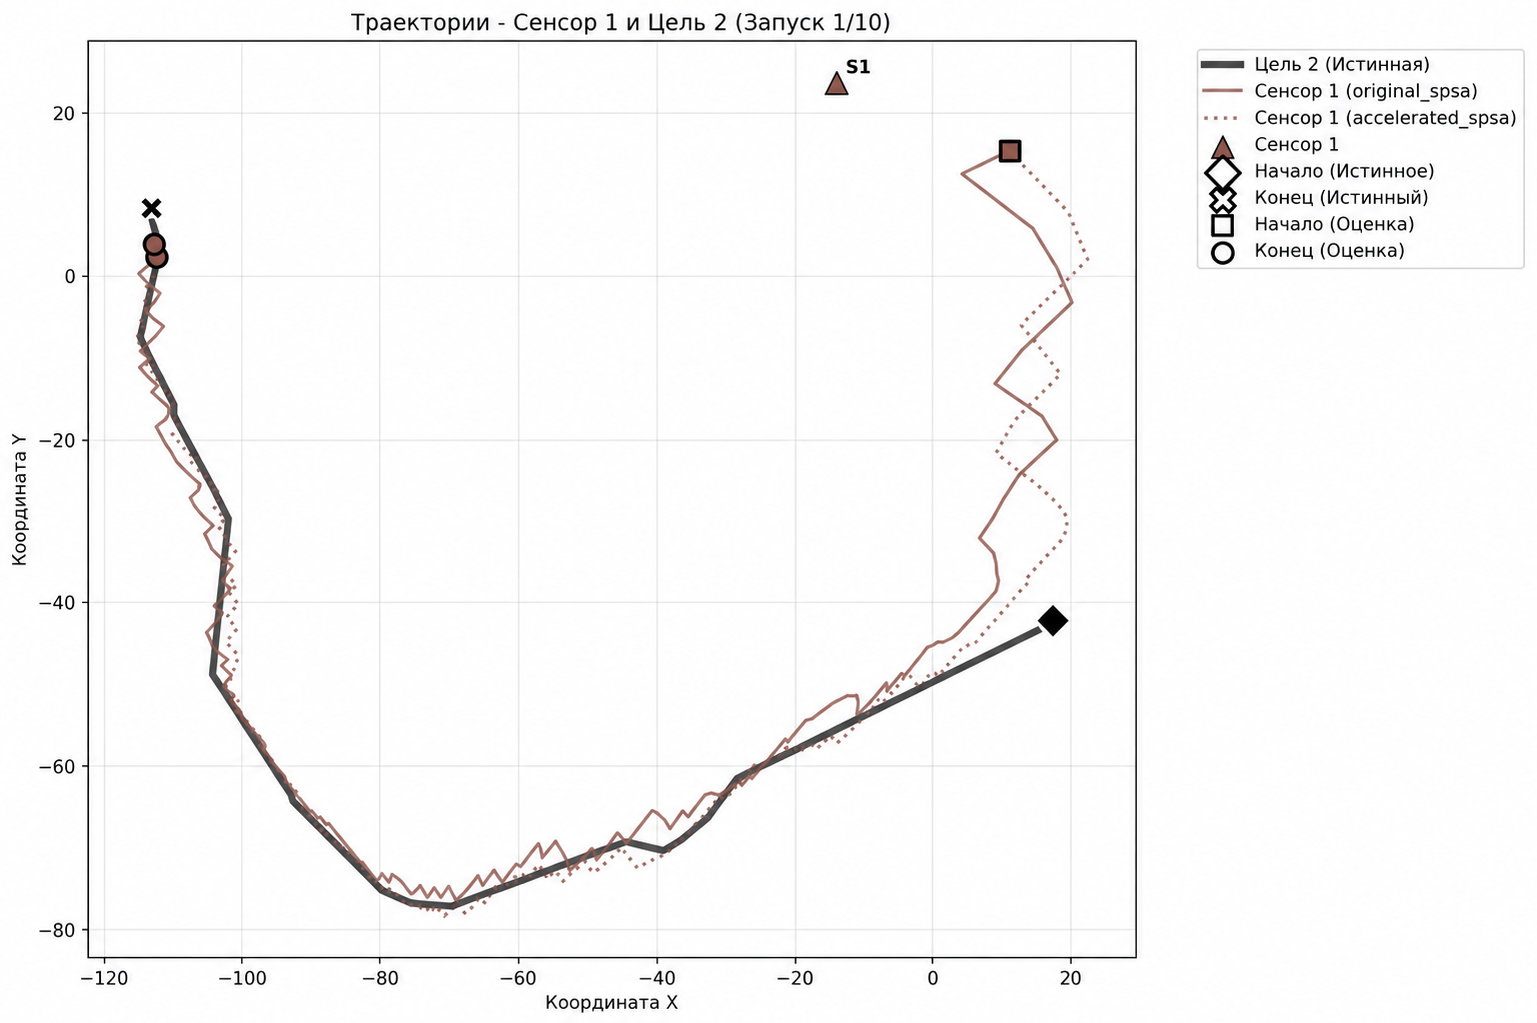
\includegraphics[width=0.58\textwidth]{Ind_left_part.png}%
        \hfill
        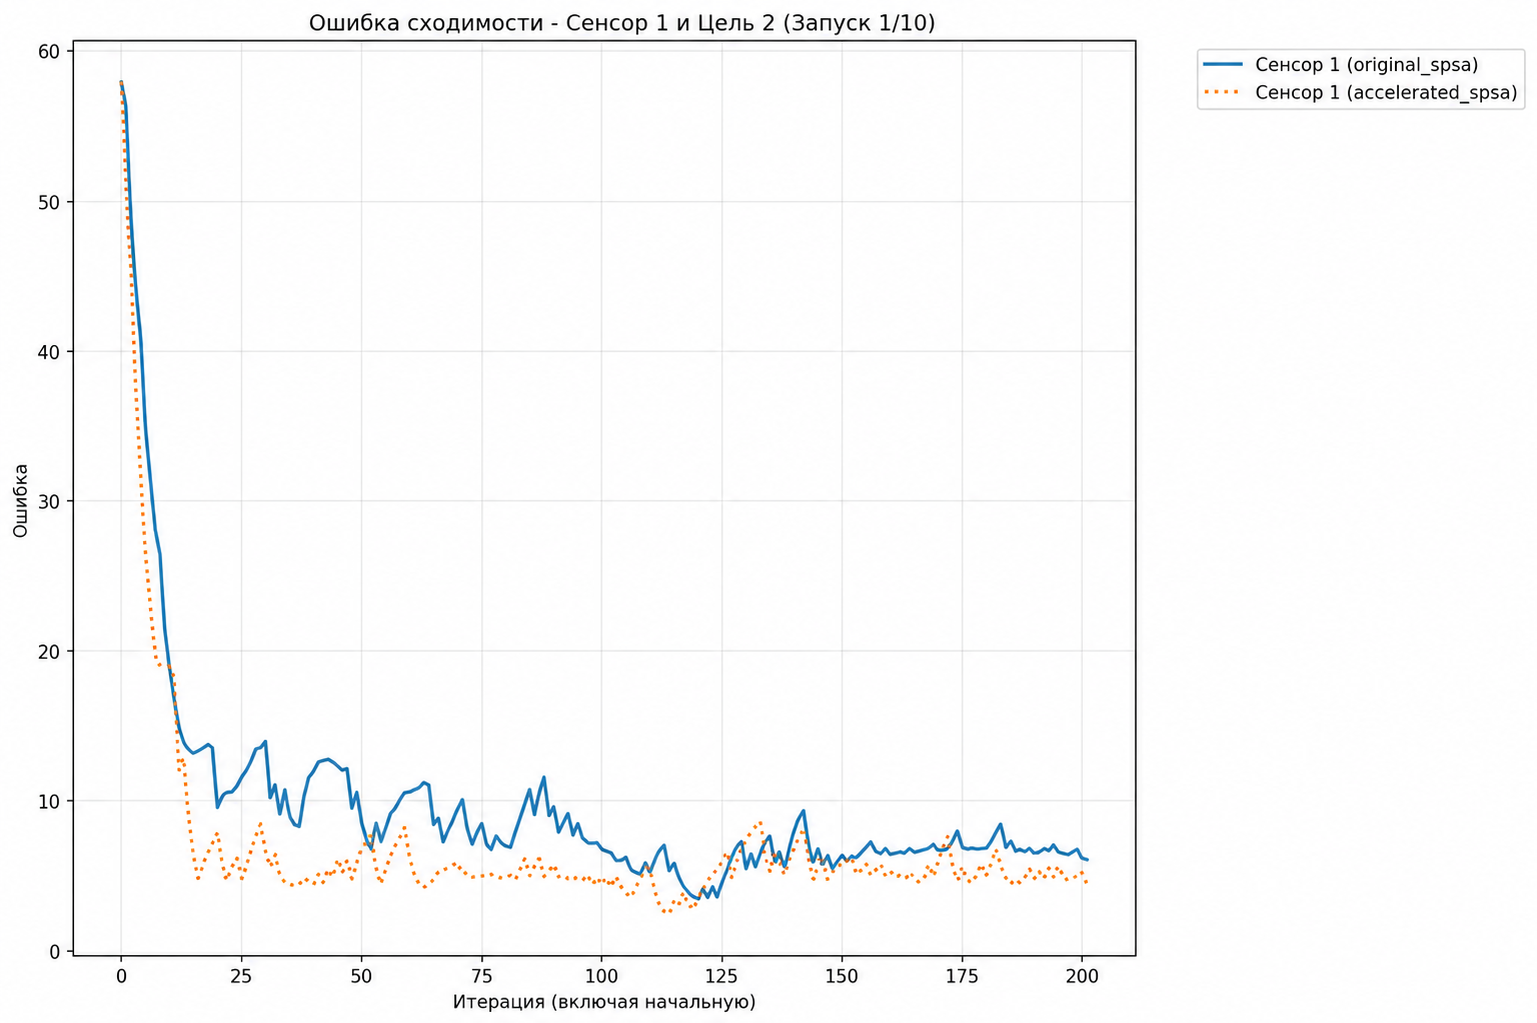
\includegraphics[width=0.58\textwidth]{Ind_right_part.png}%
    }
    \caption{Оценка конкретного сенсора за конкретной целью}
    \label{fig:specific}
\end{figure}

При выполнении нескольких запусков одной конфигурации строится агрегированный график, показывающий среднюю ошибку и доверительный интервал (стандартное отклонение) по всем запускам (рис. \ref{fig:agg}). Это позволяет оценить устойчивость алгоритмов к случайным факторам.

\begin{figure}[H]
    \centering
    \makebox[\textwidth][c]{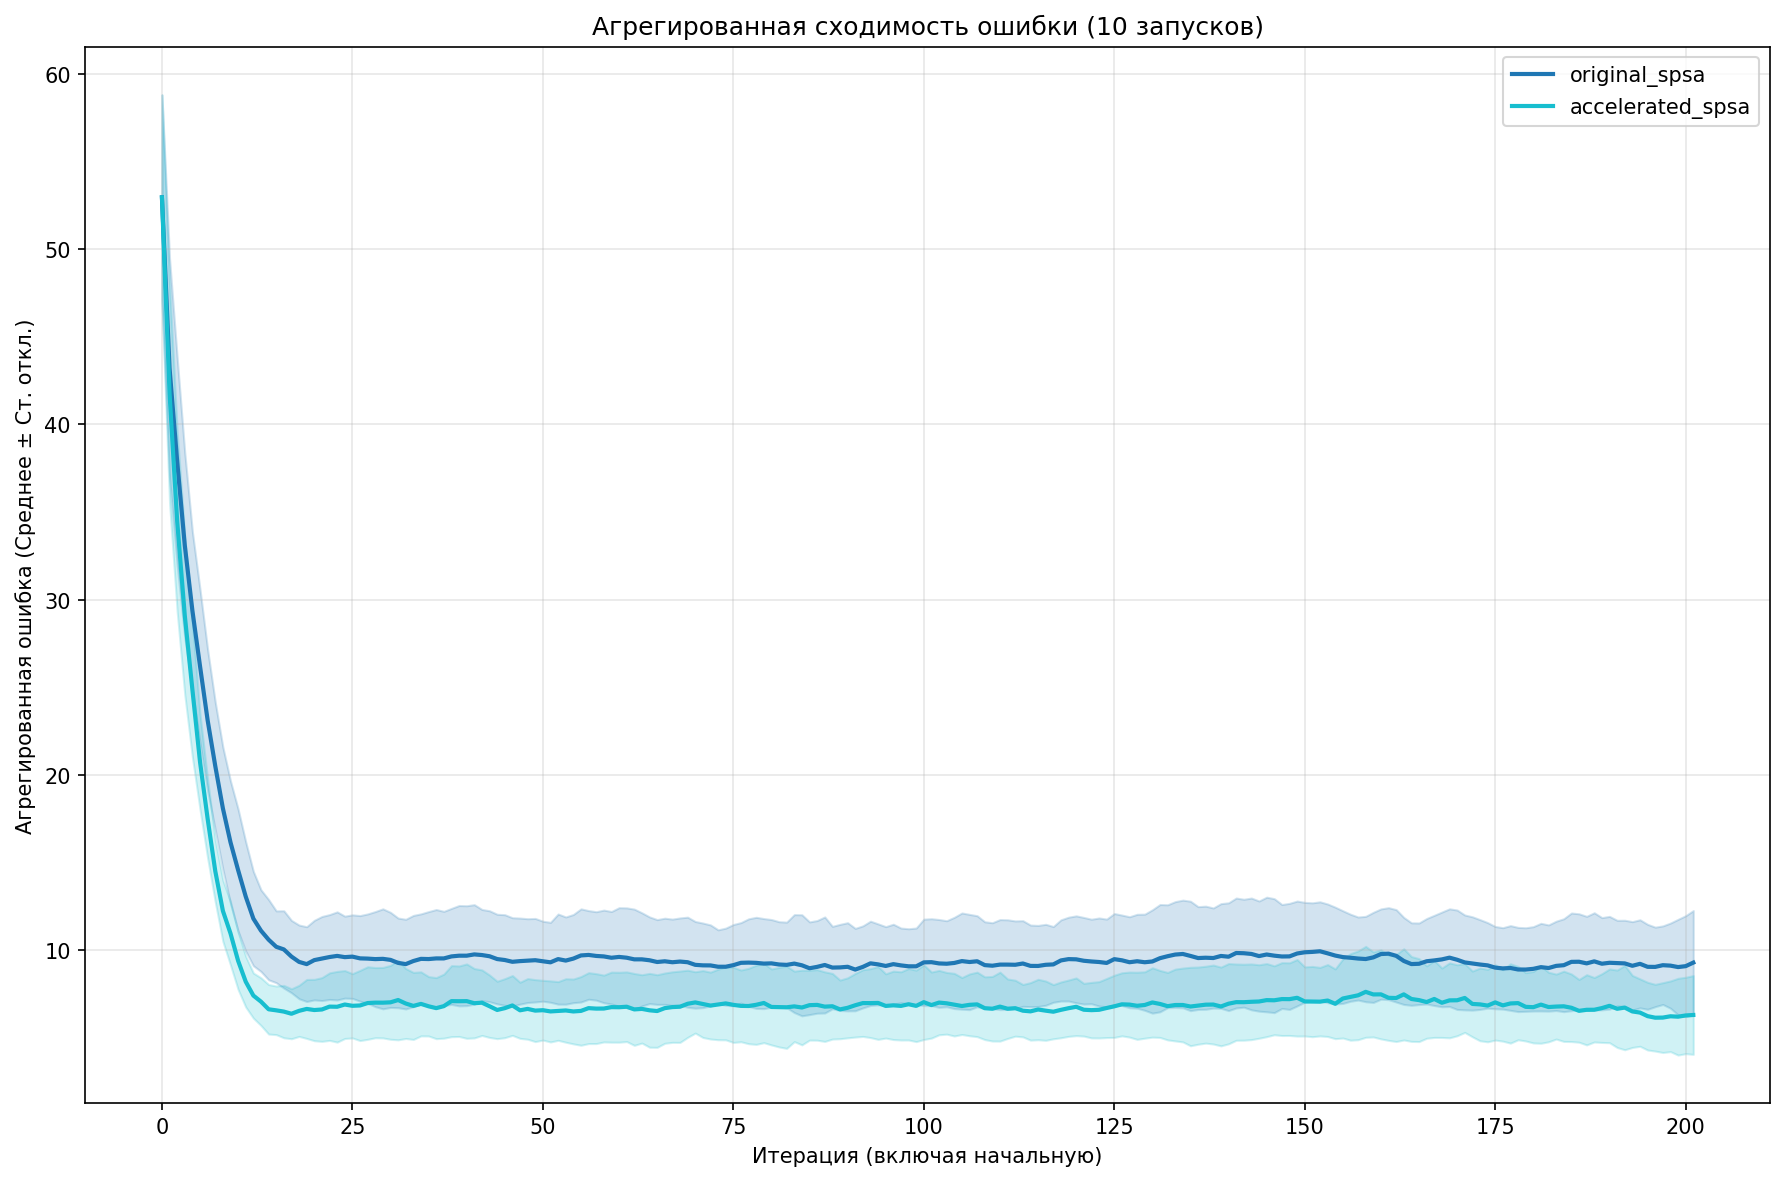
\includegraphics[width=1.05\textwidth]{agg.png}}
    \caption{Агрегированная ошибка по нескольким запускам}
    \label{fig:agg}
\end{figure}

\subsection{Реализованные алгоритмы}

В рамках работы в систему интегрированы следующие мультиагентные алгоритмы определения позиций объектов.

\paragraph{Алгоритм на основе SPSA + консенсус}


\[
\left\{
\begin{aligned}
  &\mathbf{x}_{2k}^i = \hat{\boldsymbol{\theta}}_{2k-2}^i + \beta_k^+ \boldsymbol{\Delta}_k^i, \\[0.5em]
  &\mathbf{x}_{2k-1}^i = \hat{\boldsymbol{\theta}}_{2k-2}^i - \beta_k^- \boldsymbol{\Delta}_k^i \\[0.5em]
  &\hat{\boldsymbol{\theta}}_{2k-1}^i = \hat{\boldsymbol{\theta}}_{2k-2}^i, \\[0.5em]
  &\hat{\boldsymbol{\theta}}_{2k}^i = \hat{\boldsymbol{\theta}}_{2k-1}^i - \alpha \left( \frac{y_{2k}^i - y_{2k-1}^i}{\beta_k} \mathbf{K}_k^i(\boldsymbol{\Delta}_k^i) \right. \\[0.5em]
  &\qquad \left. {} + \gamma \sum_{j \in \mathcal{N}_{2k-1}^i} b_{2k-1}^{i,j} (\tilde{\theta}_{2k-1}^{i,j} - \hat{\theta}_{2k-1}^i) \right)
\end{aligned}
\right.
\]


\paragraph{Пояснение основных шагов.}

Ниже описаны основные шаги работы алгоритма на основе SPSA, который подробно описан в статье «Simultaneous Perturbation Stochastic Approximation for Tracking Under Unknown but Bounded Disturbances». 

\begin{enumerate}

\item \textbf{Генерация возмущений.}  
На каждой итерации $k$ для каждого агента $i$ генерируется случайный вектор возмущения $\boldsymbol{\Delta}_k^i \in \mathbb{R}^d$ с симметричным распределением. Этот вектор используется для аппроксимации градиента без явного вычисления производных.

\item \textbf{Формирование точек измерения.}  
Строятся две точки:
\[
\mathbf{x}_{2k}^i = \hat{\boldsymbol{\theta}}_{2k-2}^i + \beta_k^+ \boldsymbol{\Delta}_k^i, 
\quad
\mathbf{x}_{2k-1}^i = \hat{\boldsymbol{\theta}}_{2k-2}^i - \beta_k^- \boldsymbol{\Delta}_k^i.
\]
Эти точки симметрично расположены относительно текущей оценки и используются для получения двух измерений функции.

\item \textbf{Получение наблюдений.}  
В точках $\mathbf{x}_{2k}^i$ и $\mathbf{x}_{2k-1}^i$ вычисляются (или наблюдаются) значения стохастической функции:
\[
y_{2k}^i = f_{\xi_{2k}}^i(\mathbf{x}_{2k}^i), 
\quad
y_{2k-1}^i = f_{\xi_{2k-1}}^i(\mathbf{x}_{2k-1}^i).
\]

\item \textbf{Промежуточное обновление.}  
Оценка параметра на нечётном шаге не изменяется:
\[
\hat{\boldsymbol{\theta}}_{2k-1}^i = \hat{\boldsymbol{\theta}}_{2k-2}^i.
\]
Это делается для согласования с использованием пары измерений.

\item \textbf{Оценка псевдоградиента.}  
Градиент аппроксимируется по разности наблюдений:
\[
\frac{y_{2k}^i - y_{2k-1}^i}{\beta_k} \mathbf{K}_k^i(\boldsymbol{\Delta}_k^i),
\]
где $\beta_k = \beta_k^+ + \beta_k^-$.  
Эта оценка требует всего двух измерений независимо от размерности задачи.

\item \textbf{Шаг согласования (консенсусная часть).}  
Второе слагаемое
\[
\gamma \sum_{j \in \mathcal{N}_{2k-1}^i} b_{2k-1}^{i,j} 
(\tilde{\theta}_{2k-1}^{i,j} - \hat{\theta}_{2k-1}^i)
\]
обеспечивает обмен информацией между агентами. Оно стремится согласовать оценки $\hat{\theta}^i$ с оценками соседей, полученными по шумным каналам.

\item \textbf{Обновление оценки.}  
Итоговое обновление имеет вид стохастического градиентного шага с добавлением консенсусного члена:
\[
\hat{\boldsymbol{\theta}}_{2k}^i = \hat{\boldsymbol{\theta}}_{2k-1}^i - \alpha (\text{градиентная часть} + \text{консенсусная часть}).
\]
Параметр $\alpha$ задаёт шаг обучения, а $\gamma$ — степень взаимодействия между агентами.

\end{enumerate}

\paragraph{Ускоренный алгоритм на основе SPSA + консенсус}


\[
\left\{
\begin{aligned}
  &\bar{\mathbf{x}}_k = \dfrac{1}{\gamma_{k-1} + \alpha_k(\mu - \eta)} \Big( \alpha_k \gamma_{k-1} \bar{\mathbf{z}}_{k-1} + \gamma_k \bar{\boldsymbol{\theta}}_{2k-1} \Big), \\[0.8em]
  &\bar{\mathbf{x}}_{2k} = \bar{\mathbf{x}}_k + \beta_k^+ \bar{\boldsymbol{\Delta}}_k, \quad
  \bar{\mathbf{x}}_{2k-1} = \bar{\mathbf{x}}_k - \beta_k^- \bar{\boldsymbol{\Delta}}_k, \\[0.8em]
  &\bar{\mathbf{g}}_k = \left( \dfrac{\bar{\mathbf{y}}_{2k} - \bar{\mathbf{y}}_{2k-1}}{\beta_k} \otimes \mathbf{I}_d \right) \bar{\boldsymbol{\Delta}}_k + \omega \left( \bar{\mathcal{L}}_{2k-1} \otimes E_n \right) \bar{\mathbf{x}}_k, \\[0.8em]
  &\bar{\boldsymbol{\theta}}_{2k} = \bar{\mathbf{x}}_k - h \bar{\mathbf{g}}_k, \\[0.5em]
  &\bar{\boldsymbol{\theta}}_{2k+1} = \bar{\boldsymbol{\theta}}_{2k}, \\[0.5em]
  &\bar{\mathbf{z}}_k = \dfrac{(1 - \alpha_k) \gamma_{k-1} \bar{\mathbf{z}}_{k-1} + \alpha_k (\mu - \eta) \bar{\mathbf{x}}_k - \alpha_k \bar{\mathbf{g}}_k}{\gamma_k}
\end{aligned}
\right.
\]

\paragraph{Пояснение основных шагов.}

Ниже описаны основные шаги работы ускоренного алгоритма на основе SPSA + консенсуса, который подробно описан в статье «Accelerated Consensus-Based SPSA Algorithm for Multisensor Multitarget Tracking Problem». 

\begin{enumerate}

\item \textbf{Формирование ускоренной опорной точки.}  
На каждой итерации строится точка $\bar{\mathbf{x}}_k$, которая является взвешенной комбинацией:
\begin{itemize}
    \item предыдущего вспомогательного состояния $\bar{\mathbf{z}}_{k-1}$ (накопленная информация),
    \item текущей оценки $\bar{\boldsymbol{\theta}}_{2k-1}$ (актуальное состояние).
\end{itemize}
Такое смешивание реализует эффект ускорения (аналог метода Нестерова): учитывается как «инерция» прошлых шагов, так и новое направление поиска.

\item \textbf{Генерация возмущений.}  
Формируется случайный вектор $\bar{\boldsymbol{\Delta}}_k$, компоненты которого имеют симметричное распределение.  
Он используется для аппроксимации градиента без явного вычисления производных (SPSA-подход).

\item \textbf{Формирование точек измерения.}  
Как и в классическом SPSA, строятся две симметричные точки:
\[
\bar{\mathbf{x}}_{2k} = \bar{\mathbf{x}}_k + \beta_k^+ \bar{\boldsymbol{\Delta}}_k,
\quad
\bar{\mathbf{x}}_{2k-1} = \bar{\mathbf{x}}_k - \beta_k^- \bar{\boldsymbol{\Delta}}_k.
\]
Они используются для получения двух наблюдений функции.

\item \textbf{Получение наблюдений.}  
В точках $\bar{\mathbf{x}}_{2k}$ и $\bar{\mathbf{x}}_{2k-1}$ вычисляются значения функции:
\[
\bar{\mathbf{y}}_{2k}, \quad \bar{\mathbf{y}}_{2k-1},
\]
которые могут содержать шум как измерений, так и коммуникаций между агентами.

\item \textbf{Оценка псевдоградиента.}  
Формируется оценка градиента:
\[
\left( \dfrac{\bar{\mathbf{y}}_{2k} - \bar{\mathbf{y}}_{2k-1}}{\beta_k} \otimes \mathbf{I}_d \right) \bar{\boldsymbol{\Delta}}_k,
\]
которая дополняется консенсусным слагаемым:
\[
\omega \left( \bar{\mathcal{L}}_{2k-1} \otimes E_n \right) \bar{\mathbf{x}}_k.
\]
Первое слагаемое отвечает за локальную оптимизацию (SPSA), второе — за согласование оценок между агентами сети.

\item \textbf{Обновление оценки.}  
Новая оценка параметров вычисляется как
\[
\bar{\boldsymbol{\theta}}_{2k} = \bar{\mathbf{x}}_k - h \bar{\mathbf{g}}_k.
\]
Это шаг стохастического градиентного спуска, где направление задаётся оценённым градиентом.

\item \textbf{Фиксация промежуточного состояния.}  
На следующем шаге значение не изменяется:
\[
\bar{\boldsymbol{\theta}}_{2k+1} = \bar{\boldsymbol{\theta}}_{2k}.
\]
Это необходимо для согласования с двухточечной схемой SPSA.

\item \textbf{Обновление переменной.}  
Переменная $\bar{\mathbf{z}}_k$ обновляется по рекуррентной формуле:
\[
\bar{\mathbf{z}}_k = \dfrac{(1 - \alpha_k)\gamma_{k-1}\bar{\mathbf{z}}_{k-1}
+ \alpha_k (\mu - \eta)\bar{\mathbf{x}}_k
- \alpha_k \bar{\mathbf{g}}_k}{\gamma_k}.
\]
Она аккумулирует информацию о прошлых шагах и играет роль «центра» вспомогательной квадратичной аппроксимации.

\item \textbf{Формирование новой точки.}  
На следующей итерации новая точка $\bar{\mathbf{x}}_{k+1}$ снова формируется как комбинация:
\begin{itemize}
    \item устойчивой переменной $\bar{\mathbf{z}}_k$,
    \item текущей оценки $\bar{\boldsymbol{\theta}}_{2k}$.
\end{itemize}
Это обеспечивает ускоренную сходимость за счёт контролируемого накопления импульса.


\paragraph{Распределённый фильтр Калмана}

В основе алгоритма лежит двухэтапная процедура оценивания состояния динамической системы: 
локальное обновление по измерениям и распределённое согласование оценок 
соседних агентов с помощью итераций консенсуса.

Пусть $x(t) \in \mathbb{R}$ — скалярное состояние системы, $y_i(kT)$ — измерение $i$-го агента в момент $kT$. 
Алгоритм использует $m$ обменов сообщениями между двумя последовательными измерениями. 
Оценка состояния на $i$-м узле обновляется следующим образом:

\[
\left\{
\begin{aligned}
  &\hat{x}_i(k|k) = (1 - \ell(k))\,\hat{x}_i(k|k-1) + \ell(k)\,y_i(k), \\[0.5em]
  &\hat{x}_i(k + h\delta|k) = \sum_{j=1}^{N} Q_{ij}(k,h)\;\hat{x}_j(k + (h-1)\delta|k), \qquad h = 1,\dots,m,
\end{aligned}
\right.
\]

где:
\begin{itemize}
    \item $\hat{x}_i(k|k)$ — оценка состояния на $i$-м агенте после обработки измерений в момент $k$;
    \item $\hat{x}_i(k + h\delta|k)$ — промежуточная оценка на $h$-м шаге согласования;
    \item $\delta = 1/m$ — шаг между обменами сообщениями;
    \item $\ell(k)$ — скалярный калмановский коэффициент усиления (в стационарном случае $\ell(k) \equiv \ell$);
    \item $Q(k,h)$ — стохастическая матрица согласования, совместимая с графом коммуникаций (в стационарном случае $Q(k,h) \equiv Q$);
    \item $N$ — число агентов.
\end{itemize}

\paragraph{Пояснение основных шагов.}

Ниже описаны основные шаги работы фильтра Калмана. 

\begin{itemize}

\item \textbf{Локальное обновление по измерениям.}  
Каждый агент $i$ корректирует свою предсказанную оценку $\hat{x}_i(k|k-1)$ с использованием собственного измерения $y_i(k)$:
\[
\hat{x}_i(k|k) = (1-\ell)\,\hat{x}_i(k|k-1) + \ell\,y_i(k).
\]
Это стандартный шаг калмановского обновления, не требующий коммуникаций.

\item \textbf{Распределённое согласование (консенсус).}  
Затем в течение $m$ итераций агенты обмениваются оценками с соседями и усредняют их:
\[
\hat{x}_i(k + h\delta|k) = \sum_{j=1}^{N} Q_{ij}\,\hat{x}_j(k + (h-1)\delta|k), \quad h = 1,\dots,m.
\]
Матрица $Q$ выбирается стохастической ($Q\mathbf{1}=\mathbf{1}$) и неотрицательной, а её ненулевые элементы соответствуют рёбрам графа коммуникаций. Чем больше $m$, тем точнее оценки сходятся к глобальному среднему.

\item \textbf{Предсказание на следующий шаг.}  
После завершения $m$ консенсусных итераций оценка экстраполируется вперёд по времени (для скалярного процесса с белым шумом):
\[
\hat{x}_i(k+1|k) = \hat{x}_i(k + m\delta|k),
\]
после чего цикл повторяется.

\end{itemize}
\end{enumerate}